\FloatBarrier
\subsection{Señal binaria aleatoria bipolar con diferentes valores de \(Sps\)}

Se analizó la densidad espectral de potencia (PSD) de una señal binaria aleatoria bipolar para distintos valores de muestras por símbolo (\(Sps = 1, 4, 8, 16\)). La Tabla \ref{tab:parametros_sps} resume los parámetros principales y el comportamiento temporal y espectral observado en cada caso. La Figura \ref{fig:sps_signal} presenta los resultados para \(Sps=1\), \(4\), \(8\) y \(16\), identificados individualmente en las subfiguras \ref{fig:sps1}--\ref{fig:sps16}.

En todos los ensayos se mantuvo constante la tasa de bits \(R_b\), mientras que la frecuencia de muestreo \(F_s\) aumentó proporcionalmente con \(Sps\). Por esta razón, el ancho de banda fundamental permaneció aproximadamente constante, aunque la representación temporal de la señal se hizo más detallada a medida que aumentó el sobremuestreo.

\begin{table}[H]
\caption{Comparación de la señal para diferentes valores de \(Sps\).}
\label{tab:parametros_sps}
\centering
\vspace{1mm}
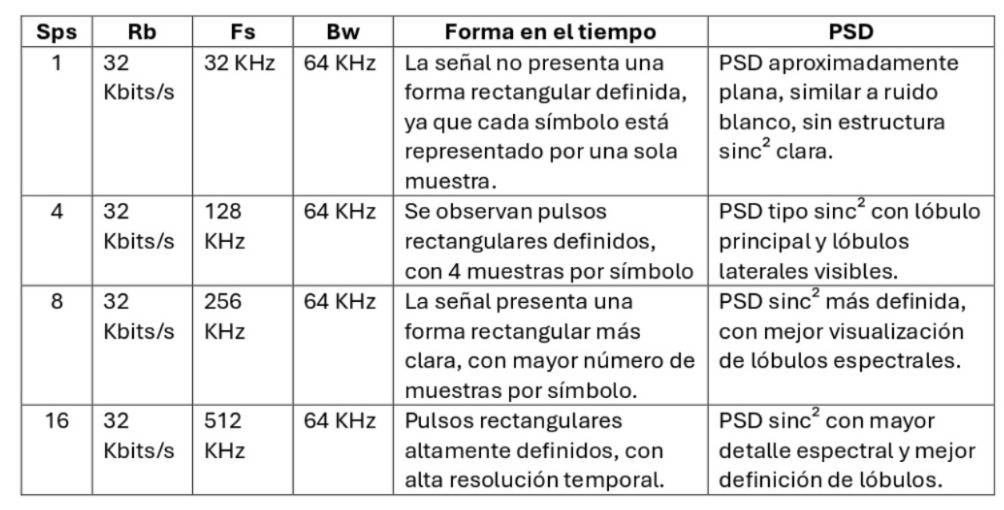
\includegraphics[width=0.95\columnwidth, trim=8 8 8 8, clip]{imagenes/tab.jpeg}
\vspace{-2mm}
\end{table}

\begin{figure}[H]
\centering
\begin{subfigure}[b]{0.48\columnwidth}
    \centering
    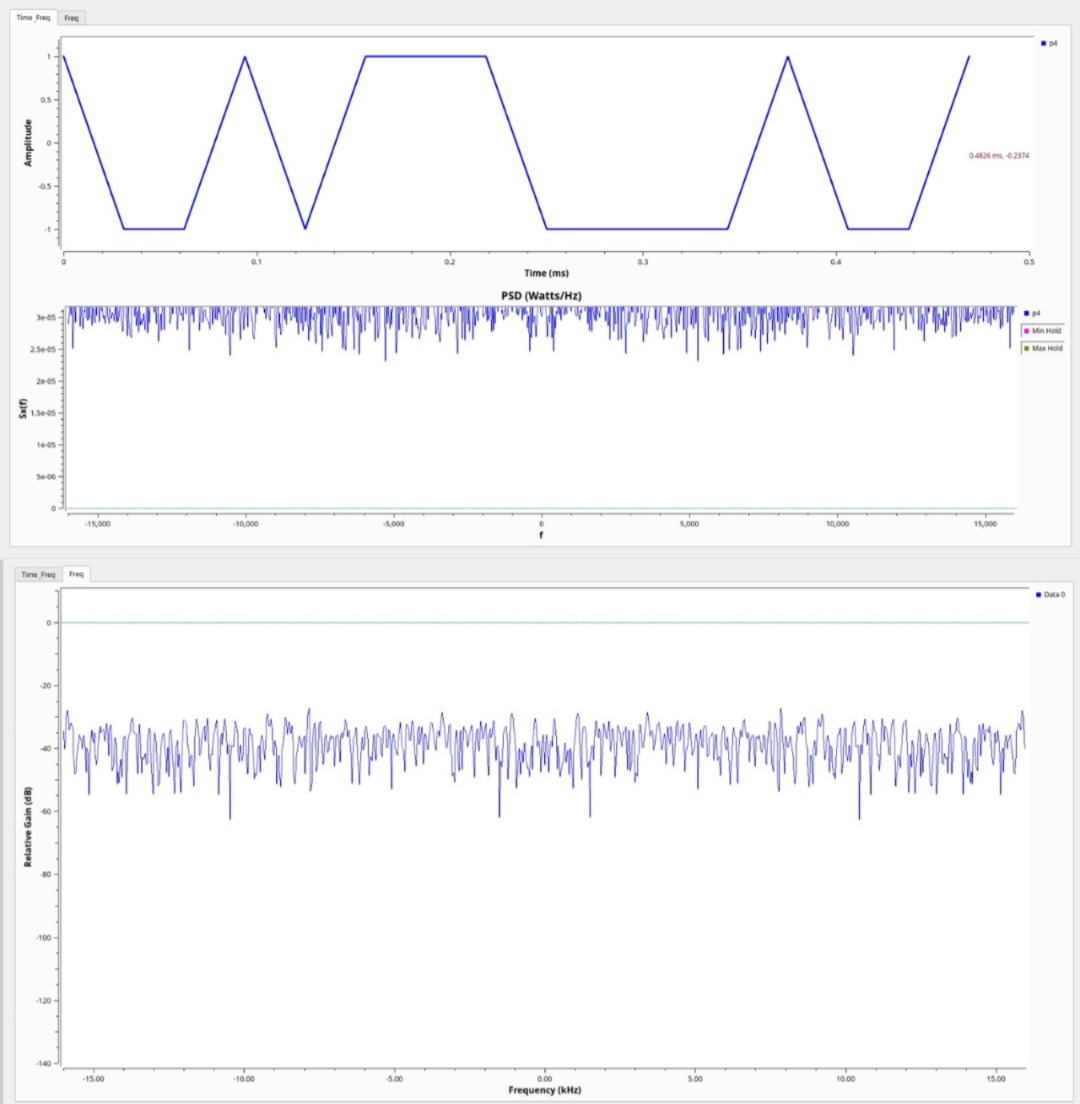
\includegraphics[width=\linewidth]{imagenes/Sps1.jpeg}
    \caption{\(Sps=1\)}
    \label{fig:sps1}
\end{subfigure}
\hfill
\begin{subfigure}[b]{0.48\columnwidth}
    \centering
    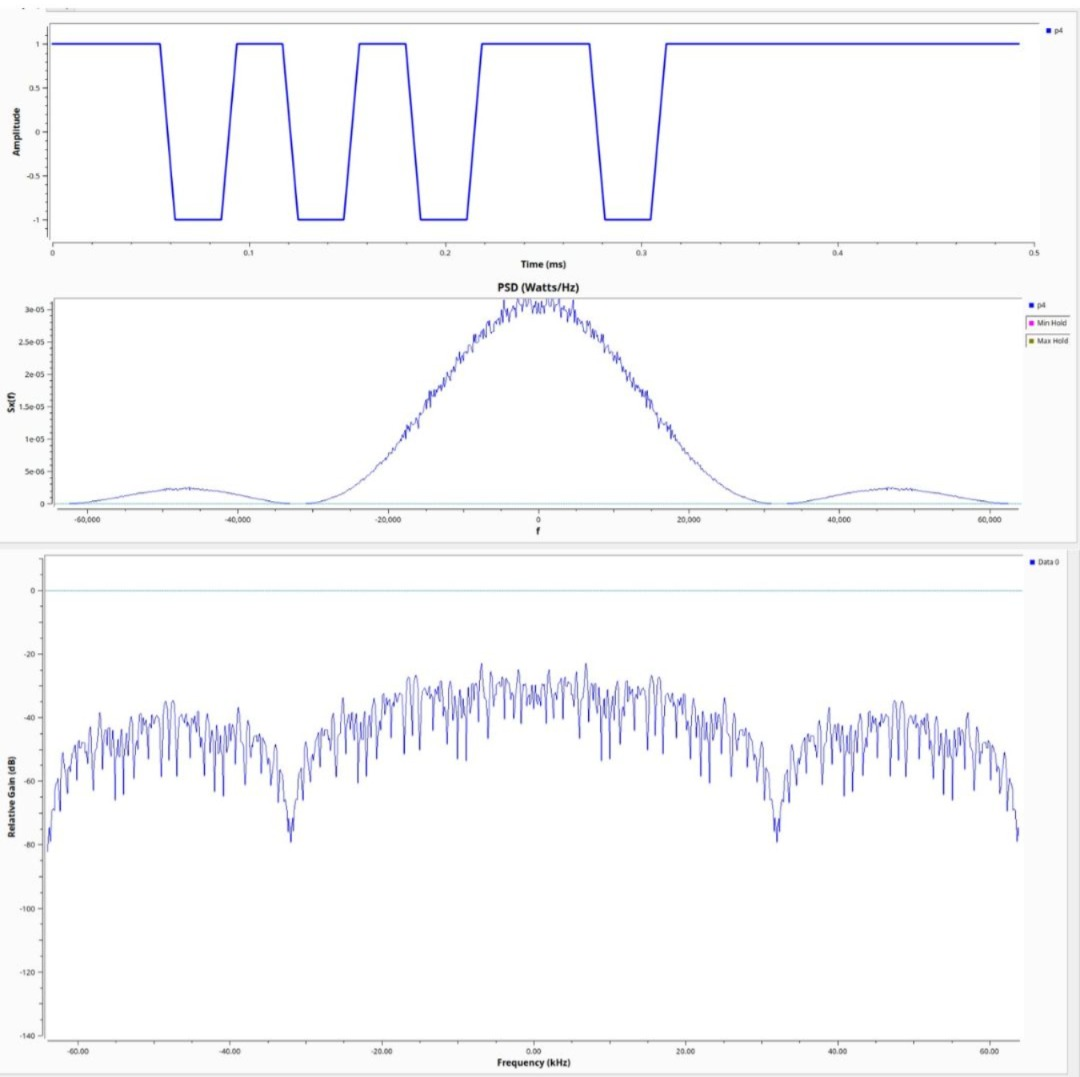
\includegraphics[width=\linewidth]{imagenes/Sps4.jpeg}
    \caption{\(Sps=4\)}
    \label{fig:sps4}
\end{subfigure}

\vspace{0.1cm}

\begin{subfigure}[b]{0.48\columnwidth}
    \centering
    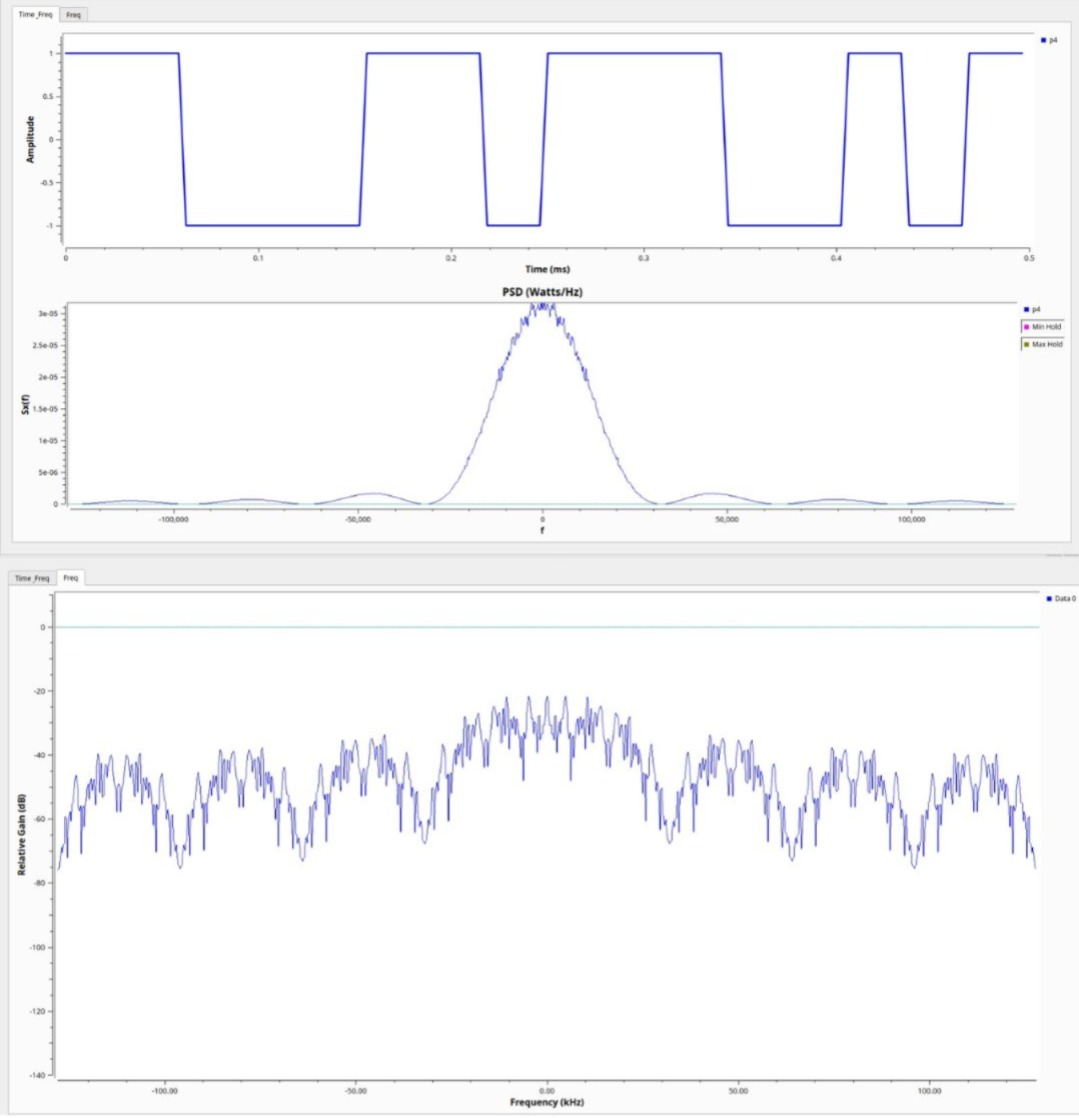
\includegraphics[width=\linewidth]{imagenes/Sps8.jpeg}
    \caption{\(Sps=8\)}
    \label{fig:sps8}
\end{subfigure}
\hfill
\begin{subfigure}[b]{0.48\columnwidth}
    \centering
    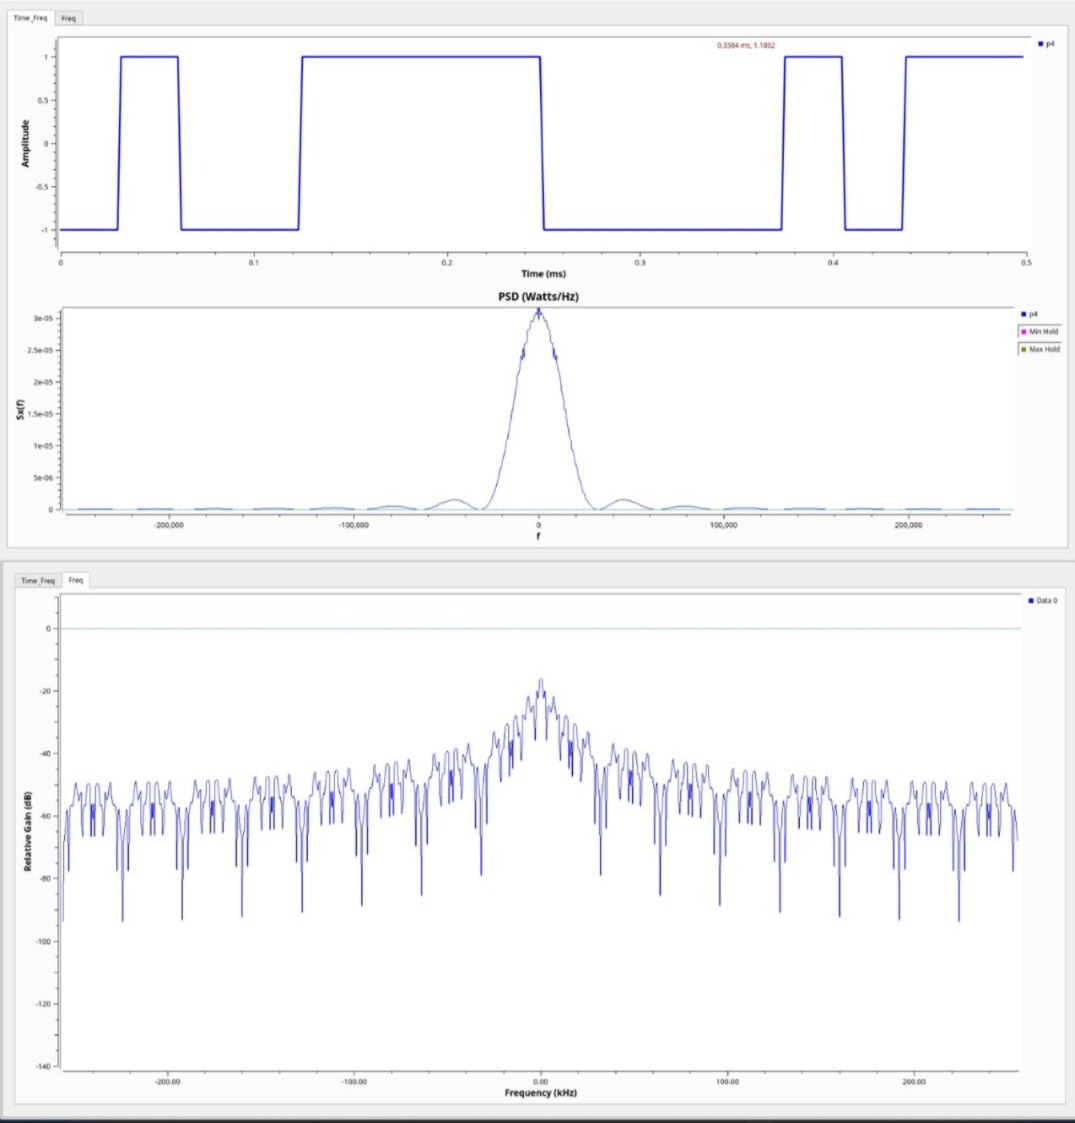
\includegraphics[width=\linewidth]{imagenes/Sps16.jpeg}
    \caption{\(Sps=16\)}
    \label{fig:sps16}
\end{subfigure}

\caption{Representación temporal y PSD de la señal binaria aleatoria bipolar para diferentes valores de \(Sps\).}
\label{fig:sps_signal}
\end{figure}

En la subfigura \ref{fig:sps1}, correspondiente a \(Sps=1\), cada símbolo queda representado por una sola muestra, por lo que la señal no exhibe una forma rectangular claramente definida y su PSD se aproxima a una distribución casi plana. En la subfigura \ref{fig:sps4}, para \(Sps=4\), ya se observan pulsos rectangulares distinguibles y aparece con mayor claridad la envolvente espectral tipo sinc\(^2\), con lóbulo principal y lóbulos laterales visibles.

En las subfiguras \ref{fig:sps8} y \ref{fig:sps16}, la forma temporal se observa con mayor resolución y la PSD presenta una definición espectral más clara. Sin embargo, el incremento de \(Sps\) no modifica la estructura espectral fundamental de la señal, sino que mejora su representación temporal y la visualización de sus componentes en frecuencia.

En consecuencia, el sobremuestreo facilita el análisis visual de la señal sin alterar la relación principal entre tasa de bits y ocupación espectral.
\FloatBarrier